% ==================///==================///==================///
% ==================/// LATEX'S STUFF
% ==================///==================///==================///

\documentclass[hungarian]{beamer}
\usepackage[T1]{fontenc}
\usepackage{babel}
\usepackage{graphicx}
\usepackage{hyperref}

\usepackage{amsfonts,amsmath,oldgerm}
\usetheme{_statale}
\usefonttheme[onlymath]{serif}

\newcommand{\testcolor}[1]{\colorbox{#1}{\textcolor{#1}{test}}~\texttt{#1}}
\newcommand{\hrefcol}[2]{\textcolor{cyan}{\href{#1}{#2}}}
\titlebackground*{assets/background}


% ==================///==================///==================///
% ==================/// SPLASH PAGE
% ==================///==================///==================///

\title{Algoritmusok I.}
\newcommand{\longauthor}{1. gyakorlat}
\author{Sipos Ágoston}
\newcommand{\correspondingauthor}{John Doe}
\newcommand{\email}{siposagoston@inf.elte.hu}
\renewcommand{\insertdate}{2026. szeptember 9.}

% ==================///==================///==================///
% ==================/// START PRESENTATION
% ==================///==================///==================///

\begin{document}
\maketitle

\section{Információk}
\begin{frame}{Információk}

\begin{itemize}
    \item Oktató: Sipos Ágoston
    \item e-mail: siposagoston@inf.elte.hu
    \item előadás weblap: \href{https://people.inf.elte.hu/kinga/algoritmusok1/seged_ea.htm}{https://people.inf.elte.hu/kinga/algoritmusok1/seged\_ea.htm}
    \item további anyagok: Canvas (pl. ezek a slide-ok)
    \item tankönyv: Cormen, Leiserson, Rivest, Stein: Új Algoritmusok, Scolar Kiadó, 2003, online tananyag: \href{https://tamop412.elte.hu/tananyagok/algoritmusok/}{https://tamop412.elte.hu/tananyagok/algoritmusok/}
\end{itemize}

\end{frame}

\begin{frame}{Követelmények}
\begin{itemize}
    \item Személyes részvétel a gyakorlatokon (legfeljebb 3 hiányzással)
    \item Heti Canvas kvízek
    \begin{itemize}
        \item Többször is kitölthetők!
        \item Legalább 70\% kell
    \end{itemize}
    \item 2 zárthelyi dolgozat
    \begin{itemize}
        \item Előadás időpontjában! (évfolyam-ZH)
        \item Mindkét ZH 50 pontos; minimumpontszám: 15-15
    \end{itemize}
    \item Összpontszám: a két ZH pontszáma + maximum 15 szorgalmi pont
    \item Ponthatárok: 40-től 2, 55-től 3, 70-től 4, 85-től 5 (a ketteshez a 2 ZH-ból már meg kell lennie a 40 pontnak!)
    \item ZH-k várható időpontja: október 14., december 9.
\end{itemize}
\end{frame}

\begin{frame}{Tervezett tanmenet}
\begin{enumerate}
    \item Bevezetés; buborék- és kiválasztásos rendezés
    \item Aszimptotika. Verem és sor
    \item Láncolt listák
    \item Kétirányú és ciklikus láncolt listák
    \item Beszúró-, összefésülő és gyorsrendezés
    \item Gyakorlás (ZH hete)
    \item ZH feladatok megoldásai
    \vspace{3mm}
    \item Bináris fa
    \item Bináris keresőfa
    \item Kupac, prioritásos sor
    \item Hasító táblák
    \item Rendezés lineáris időben
    \item Gyakorlás
\end{enumerate}
\end{frame}

\section{Bevezetés}

\begin{frame}{Mi az algoritmus?}
Algoritmusnak nevezünk bármilyen \textbf{jól definiált} számítási eljárást, amely \textbf{bemenetként} bizonyos értéket vagy értékeket kap és \textbf{kimenetként} bizonyos értéket vagy értékeket állít elő (\textbf{véges időn belül}).

\vspace{5mm}

Másképp, olyan számítási lépések sorozata, amelyek a bemenetet átalakítják kimenetté.

{\scriptsize (Cormen, Leiserson, Rivest, Stein: Új Algoritmusok}
\vspace{5mm}
\begin{itemize}
    \item De az a véges idő nem mindegy, hogy mennyi
\end{itemize}
\end{frame}

\begin{frame}{Műveletigény}
\begin{itemize}
    \item Annak mérőszáma, hogy az algoritmus során mennyi \textit{elemi műveletet} hajtunk végre
    \item Elemi művelet pl. összeadás, szorzás, összehasonlítás, ...
    \item De az, hogy mennyi műveletet hajtunk végre, nagyon függ a bemenettől. Szokásos mérőszámok:
    \begin{itemize}
        \item $MT(n)$ egy $n$ méretű bemeneten \textit{maximum} ennyi műveletet hajt végre az algoritmus
        \item $mT(n)$ egy $n$ méretű bemeneten \textit{legalább} ennyi műveletet hajt végre az algoritmus
        \item $AT(n)$ egy $n$ méretű bemeneten \textit{átlagosan} (várható értékben) ennyi műveletet hajt végre az algoritmus
    \end{itemize}
    \item Általában nem is akarjuk pontosan tudni, csak a nagyságrendjét: \textit{aszimptotika}
\end{itemize}
\end{frame}

\begin{frame}{Aszimptotika}
Pl. aszimptotikus felső becslés ($\mathcal{O}$): $\exists N \in \mathbb{N}: \forall n>N: \exists d \in \mathbb{R}: d \cdot g(n) > f(n)$ ekkor $g$ aszimp. felső becslése $f$-nek. (Jele: $f = \mathcal{O}(g)$)

Például $n^2 + 3n + 2$-nek aszimptotikus felső becslése $n^2$, pl. $d = 2$, $N = 4$ választással. (más választás is lehetséges)

Általában $d$-vel és $N$-nel sem foglalkozunk.

Aszimptotikus alsó becslés analóg módon (jele $\Omega$). Aszimptotikus alsó és felső becslés, ha különböző konstansokkal mindkettő igaz (jele $\Theta$)


Demó: \href{https://www.desmos.com/calculator/goailfzscl}{https://www.desmos.com/calculator/goailfzscl}
\end{frame}

\begin{frame}[fragile]{Példa}


\begin{columns}

\begin{column}{0.5\linewidth}
\begin{verbatim}
def fibonacci_naive(n):
    if n <= 0:
        return 0
    elif n == 1:
        return 1
    return fibonacci_naive(n - 1) + \
        fibonacci_naive(n - 2)
\end{verbatim}
\end{column}
\begin{column}{0.5\linewidth}
\begin{verbatim}
def fibonacci_iterative(n):
    if n <= 0:
        return 0
    elif n == 1:
        return 1
    a, b = 0, 1
    for _ in range(2, n + 1):
        a, b = b, a + b
    return b
\end{verbatim}

\end{column}

\end{columns}
    
\end{frame}

\section{Polinom kiértékelése}

\begin{frame}{Feladat}
Adott $a_n, a_{n-1}, \dots, a_1, a_0$ és $x$ esetén értékeljük ki a

$$\sum_{i=0}^n a_i \cdot x^i$$

polinomot.

\end{frame}

\begin{frame}{Naiv algoritmus}

Legyenek az együtthatók egy $A$ tömbben adottak (bemenet). A tömb hossza $N+1$, ha $0$-tól indexelünk, akkor A[i] = $a_i$ éppen. \pause

\begin{columns}

\begin{column}{0.5\linewidth}
\begin{figure}
    \centering
    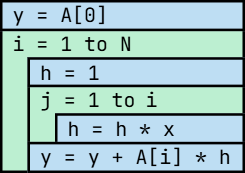
\includegraphics[width=0.8\linewidth]{assets/polinom1.png}
    \caption{polinom kiértékelése}
    \label{fig:poly1}
\end{figure}
\end{column}
\begin{column}{0.5\linewidth}

Eredmény a lefutás után y-ban van. \pause

Műveletek száma:

Összeadás: külső ciklusban 1, tehát össz. N

Szorzás: belső ciklusban 1, az a külső ciklusmagban összesen N, plusz még egy a belső cikluson kívül, tehát összesen N*(N+1)

Tfh. összeadás és szorzás egyforma költség: $N+N*(N+1)$ művelet összesen.

Kifejtve: $N^2 + 2N$

Aszimptotikusan $\Theta(N^2)$

\end{column}

\end{columns}
\end{frame}

\begin{frame}{Második megközelítés}

A naiv algoritmus $h$-t mindig újra kiszámolta, pedig az előzőből egyszerűen számolható.


\begin{columns}

\begin{column}{0.5\linewidth}

\begin{figure}
    \centering
    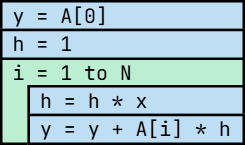
\includegraphics[width=0.8\linewidth]{assets/polinom2.png}
    \caption{polinom kiértékelése}
    \label{fig:poly2}
\end{figure}
\end{column}
\begin{column}{0.5\linewidth}
\pause
Műveletek száma:

Összeadás: ciklusban 1, tehát össz. N

Szorzás: ciklusban 2, tehát össz. 2N

Tfh. összeadás és szorzás egyforma költség: $3N$ művelet összesen.

Aszimptotikusan $\Theta(N)$

\end{column}

\end{columns}
    
\end{frame}

\begin{frame}{Harmadik megközelítés (Horner-séma)}

Írjuk át a polinomot $(\dots((a_n x + a_{n-1})x + a_{n-2})x + \dots + a_1)x+a_0$ alakra. Látható, hogy ez egy ekvivalens átalakítás.

Ebből adódik az alábbi algoritmus:

\begin{columns}

\begin{column}{0.5\linewidth}

\begin{figure}
    \centering
    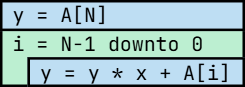
\includegraphics[width=0.8\linewidth]{assets/polinom3.png}
    \caption{polinom kiértékelése}
    \label{fig:poly3}
\end{figure}
\end{column}
\begin{column}{0.5\linewidth}
\pause
Műveletek száma:

Összeadás: ciklusban 1, tehát össz. N

Szorzás: ciklusban 1, tehát össz. N

Tfh. összeadás és szorzás egyforma költség: $2N$ művelet összesen.

Aszimptotikusan $\Theta(N)$

Megjegyzés: aszimptotikusan ugyanannyi mint az előző, de az $3N$ ez pedig $2N$ tehát egyértelműen jobb. Polinom műv.ig. esetén tehát előfordul, hogy a főegyütthatóra is kíváncsiak vagyunk, nem csak a fokszámra.

\end{column}

\end{columns}
    
\end{frame}

\section{Rendezési probléma}

\begin{frame}{Feladat}

Alapprobléma: adott egy számsorozat, rendezzük növekvő sorrendbe.

Pl. $(31,41,59,26,41,58) \rightarrow  (26,31,41,41,58,59)$

Több algoritmust is vizsgálni fogunk a félév során.

Különféle helyzetekben más-más algoritmus lehet a ,,legjobb''.

\end{frame}

\begin{frame}{Stabilitás}

Egy rendező algoritmus stabil, ha az egyenlő elemek relatív sorrendjét nem változtatja meg.

(Ha csak számok vannak a tömbben, akkor nem túl érdekes, de ha összetett adatok, amiket az egyik mezőjük, egy szám, alapján rendezünk, akkor már fontos lehet.)

Pl. $(1,3,4,2a,8,2b) \rightarrow  (1,2a,2b,3,4,8)$ és nem $(1,2b,2a,3,4,8)$

\end{frame}

\begin{frame}[t]{Buborékrendezés}

Ötlet: nézzük meg a szomszédos elemeket, ha fordított sorrendben vannak, cseréljük meg. Csináljuk ezt addig, amíg rendezett lesz a tömb.

\begin{tabular}{|c|c|c|c|c|c|}
    \hline
    31 & 41 & 59 & 26 & 41 & 58 \\
    \hline
\end{tabular}

\end{frame}

\begin{frame}[t]{Javított buborékrendezés}

Ötlet: ha a tömb egy része már rendezett, akkor ne végezzünk felesleges összehasonlításokat

\begin{tabular}{|c|c|c|c|c|c|}
    \hline
    31 & 41 & 59 & 26 & 41 & 58 \\
    \hline
\end{tabular}

\end{frame}

\begin{frame}[t]{Maximumkiválasztásos rendezés}

Ötlet: válasszuk ki a legnagyobb elemet, és tegyük az utolsó helyre. Ezután keressük meg a többi elem közül a legnagyobbat és így tovább.

\begin{tabular}{|c|c|c|c|c|c|}
    \hline
    31 & 41 & 59 & 26 & 41 & 58 \\
    \hline
\end{tabular}

\end{frame}

\end{document}
